% Options for packages loaded elsewhere
% Options for packages loaded elsewhere
\PassOptionsToPackage{unicode}{hyperref}
\PassOptionsToPackage{hyphens}{url}
\PassOptionsToPackage{dvipsnames,svgnames,x11names}{xcolor}
%
\documentclass[
  letterpaper,
  DIV=11,
  numbers=noendperiod]{scrartcl}
\usepackage{xcolor}
\usepackage{amsmath,amssymb}
\setcounter{secnumdepth}{-\maxdimen} % remove section numbering
\usepackage{iftex}
\ifPDFTeX
  \usepackage[T1]{fontenc}
  \usepackage[utf8]{inputenc}
  \usepackage{textcomp} % provide euro and other symbols
\else % if luatex or xetex
  \usepackage{unicode-math} % this also loads fontspec
  \defaultfontfeatures{Scale=MatchLowercase}
  \defaultfontfeatures[\rmfamily]{Ligatures=TeX,Scale=1}
\fi
\usepackage{lmodern}
\ifPDFTeX\else
  % xetex/luatex font selection
\fi
% Use upquote if available, for straight quotes in verbatim environments
\IfFileExists{upquote.sty}{\usepackage{upquote}}{}
\IfFileExists{microtype.sty}{% use microtype if available
  \usepackage[]{microtype}
  \UseMicrotypeSet[protrusion]{basicmath} % disable protrusion for tt fonts
}{}
\makeatletter
\@ifundefined{KOMAClassName}{% if non-KOMA class
  \IfFileExists{parskip.sty}{%
    \usepackage{parskip}
  }{% else
    \setlength{\parindent}{0pt}
    \setlength{\parskip}{6pt plus 2pt minus 1pt}}
}{% if KOMA class
  \KOMAoptions{parskip=half}}
\makeatother
% Make \paragraph and \subparagraph free-standing
\makeatletter
\ifx\paragraph\undefined\else
  \let\oldparagraph\paragraph
  \renewcommand{\paragraph}{
    \@ifstar
      \xxxParagraphStar
      \xxxParagraphNoStar
  }
  \newcommand{\xxxParagraphStar}[1]{\oldparagraph*{#1}\mbox{}}
  \newcommand{\xxxParagraphNoStar}[1]{\oldparagraph{#1}\mbox{}}
\fi
\ifx\subparagraph\undefined\else
  \let\oldsubparagraph\subparagraph
  \renewcommand{\subparagraph}{
    \@ifstar
      \xxxSubParagraphStar
      \xxxSubParagraphNoStar
  }
  \newcommand{\xxxSubParagraphStar}[1]{\oldsubparagraph*{#1}\mbox{}}
  \newcommand{\xxxSubParagraphNoStar}[1]{\oldsubparagraph{#1}\mbox{}}
\fi
\makeatother


\usepackage{longtable,booktabs,array}
\newcounter{none} % for unnumbered tables
\usepackage{calc} % for calculating minipage widths
% Correct order of tables after \paragraph or \subparagraph
\usepackage{etoolbox}
\makeatletter
\patchcmd\longtable{\par}{\if@noskipsec\mbox{}\fi\par}{}{}
\makeatother
% Allow footnotes in longtable head/foot
\IfFileExists{footnotehyper.sty}{\usepackage{footnotehyper}}{\usepackage{footnote}}
\makesavenoteenv{longtable}
\usepackage{graphicx}
\makeatletter
\newsavebox\pandoc@box
\newcommand*\pandocbounded[1]{% scales image to fit in text height/width
  \sbox\pandoc@box{#1}%
  \Gscale@div\@tempa{\textheight}{\dimexpr\ht\pandoc@box+\dp\pandoc@box\relax}%
  \Gscale@div\@tempb{\linewidth}{\wd\pandoc@box}%
  \ifdim\@tempb\p@<\@tempa\p@\let\@tempa\@tempb\fi% select the smaller of both
  \ifdim\@tempa\p@<\p@\scalebox{\@tempa}{\usebox\pandoc@box}%
  \else\usebox{\pandoc@box}%
  \fi%
}
% Set default figure placement to htbp
\def\fps@figure{htbp}
\makeatother





\setlength{\emergencystretch}{3em} % prevent overfull lines

\providecommand{\tightlist}{%
  \setlength{\itemsep}{0pt}\setlength{\parskip}{0pt}}



 


\usepackage{booktabs}
\usepackage{longtable}
\usepackage{array}
\usepackage{multirow}
\usepackage{wrapfig}
\usepackage{float}
\usepackage{colortbl}
\usepackage{pdflscape}
\usepackage{tabu}
\usepackage{threeparttable}
\usepackage{threeparttablex}
\usepackage[normalem]{ulem}
\usepackage{makecell}
\usepackage{xcolor}
\KOMAoption{captions}{tableheading}
\makeatletter
\@ifpackageloaded{caption}{}{\usepackage{caption}}
\AtBeginDocument{%
\ifdefined\contentsname
  \renewcommand*\contentsname{Table of contents}
\else
  \newcommand\contentsname{Table of contents}
\fi
\ifdefined\listfigurename
  \renewcommand*\listfigurename{List of Figures}
\else
  \newcommand\listfigurename{List of Figures}
\fi
\ifdefined\listtablename
  \renewcommand*\listtablename{List of Tables}
\else
  \newcommand\listtablename{List of Tables}
\fi
\ifdefined\figurename
  \renewcommand*\figurename{Figure}
\else
  \newcommand\figurename{Figure}
\fi
\ifdefined\tablename
  \renewcommand*\tablename{Table}
\else
  \newcommand\tablename{Table}
\fi
}
\@ifpackageloaded{float}{}{\usepackage{float}}
\floatstyle{ruled}
\@ifundefined{c@chapter}{\newfloat{codelisting}{h}{lop}}{\newfloat{codelisting}{h}{lop}[chapter]}
\floatname{codelisting}{Listing}
\newcommand*\listoflistings{\listof{codelisting}{List of Listings}}
\makeatother
\makeatletter
\makeatother
\makeatletter
\@ifpackageloaded{caption}{}{\usepackage{caption}}
\@ifpackageloaded{subcaption}{}{\usepackage{subcaption}}
\makeatother
\usepackage{bookmark}
\IfFileExists{xurl.sty}{\usepackage{xurl}}{} % add URL line breaks if available
\urlstyle{same}
\hypersetup{
  pdftitle={MIxS-UX Survey on experiences on the use and development of MIxS metadata standards},
  pdfauthor={James A. Fellows Yates},
  colorlinks=true,
  linkcolor={blue},
  filecolor={Maroon},
  citecolor={Blue},
  urlcolor={Blue},
  pdfcreator={LaTeX via pandoc}}


\title{MIxS-UX Survey on experiences on the use and development of MIxS
metadata standards}
\author{James A. Fellows Yates}
\date{2026-06-03}
\begin{document}
\maketitle

\renewcommand*\contentsname{Table of contents}
{
\setcounter{tocdepth}{3}
\tableofcontents
}

\subsection{Introduction}\label{introduction}

This anonymous survey has been designed to get an overview of current
awareness and experiences in using the `Minimal Information About (X)
Any Sequence' or `MIxS' suite of metadata checklists designed by the
Genomic Standards Consortium (GSC) for the reporting of nucleic acid
sequencing data.

The MIxS checklists aim to greatly enrich the contextual annotation
around DNA and RNA data to improve accessibility, promote effective
re-use, and maximise scientific (re-)discovery from the vast amount of
genomic data being produced by scientists today.

The results from this survey will be used to help guide the
NFDI4Microbiota `MIxS-UX' FlexFund project improve the documentation
around MIxS.

\begin{verbatim}
R version 4.4.1 (2024-06-14)
Platform: x86_64-pc-linux-gnu
Running under: Ubuntu 24.04.4 LTS

Matrix products: default
BLAS:   /usr/lib/x86_64-linux-gnu/blas/libblas.so.3.12.0 
LAPACK: /usr/lib/x86_64-linux-gnu/lapack/liblapack.so.3.12.0

locale:
 [1] LC_CTYPE=en_GB.UTF-8       LC_NUMERIC=C              
 [3] LC_TIME=en_GB.UTF-8        LC_COLLATE=en_GB.UTF-8    
 [5] LC_MONETARY=en_GB.UTF-8    LC_MESSAGES=en_GB.UTF-8   
 [7] LC_PAPER=en_GB.UTF-8       LC_NAME=C                 
 [9] LC_ADDRESS=C               LC_TELEPHONE=C            
[11] LC_MEASUREMENT=en_GB.UTF-8 LC_IDENTIFICATION=C       

time zone: Europe/Berlin
tzcode source: system (glibc)

attached base packages:
[1] stats     graphics  grDevices utils     datasets  methods   base     

other attached packages:
[1] patchwork_1.2.0  kableExtra_1.4.0 forcats_1.0.0    tidyr_1.3.1     
[5] stringr_1.5.1    janitor_2.2.1    ggplot2_3.5.1    dplyr_1.1.4     
[9] readr_2.1.5     

loaded via a namespace (and not attached):
 [1] gtable_0.3.5      jsonlite_1.8.8    compiler_4.4.1    tidyselect_1.2.1 
 [5] xml2_1.3.6        snakecase_0.11.1  systemfonts_1.2.3 scales_1.3.0     
 [9] yaml_2.3.8        fastmap_1.1.1     R6_2.5.1          generics_0.1.3   
[13] knitr_1.50        tibble_3.2.1      munsell_0.5.1     svglite_2.1.3    
[17] lubridate_1.9.3   pillar_1.9.0      tzdb_0.4.0        rlang_1.1.6      
[21] utf8_1.2.4        stringi_1.8.3     xfun_0.52         viridisLite_0.4.2
[25] timechange_0.3.0  cli_3.6.5         withr_3.0.0       magrittr_2.0.3   
[29] digest_0.6.35     grid_4.4.1        rstudioapi_0.16.0 hms_1.1.3        
[33] lifecycle_1.0.4   vctrs_0.6.5       evaluate_0.23     glue_1.8.0       
[37] fansi_1.0.6       colorspace_2.1-0  purrr_1.0.2       rmarkdown_2.27   
[41] tools_4.4.1       pkgconfig_2.0.3   htmltools_0.5.8.1
\end{verbatim}

\subsection{Key Takeaways}\label{key-takeaways}

\begin{enumerate}
\def\labelenumi{\arabic{enumi}.}
\tightlist
\item
  Most responders are interested in both using and contributing to MIxS.
\item
  Most responders were working at a post-doctoral level or higher.
\item
  The MIxS GitHub repository and/or the associated website is the
  primary source of information on MIxS.
\item
  Familiarity with core MIxS concepts by responders is mixed.
\item
  Primary blockers to new contributors are lack of time or not knowing
  how to contribute.
\item
  MIMS, MIMAG, and MIMARK checklists were most popular, and good targets
  for documentation examples and training material.
\end{enumerate}

\subsection{Survey Structure}\label{survey-structure}

The survey ran from 2026-02-18 to 2026-03-24. An optional raffle was
offered, with 3 small prizes (stickers, and other GSC merchandise)
allocated. The survey was hosted on \url{https://tally.so}, and directly
advertised on:

\begin{itemize}
\tightlist
\item
  NFDI4Microbiota mailing list
\item
  Genomic Standard Consortium Slack
\item
  GSC mailing list
\item
  LinkedIn
\item
  Mastodon
\item
  ISBA Slack
\item
  Bluesky
\end{itemize}

Questions were grouped into the following sections:

\begin{itemize}
\tightlist
\item
  Demographic questions
\item
  Basic questions
\item
  Usage of MIxS
\item
  Knowledge of MIxS
\item
  Contributing to MixS
\item
  Technical Questions
\item
  Wider context
\end{itemize}

There were \textbf{56} responses in total.

\subsection{Survey Responses}\label{survey-responses}

\subsubsection{Demographics}\label{demographics}

To get a better idea of who the responders were, we can look at the
geographic distribution of responders.

\pandocbounded{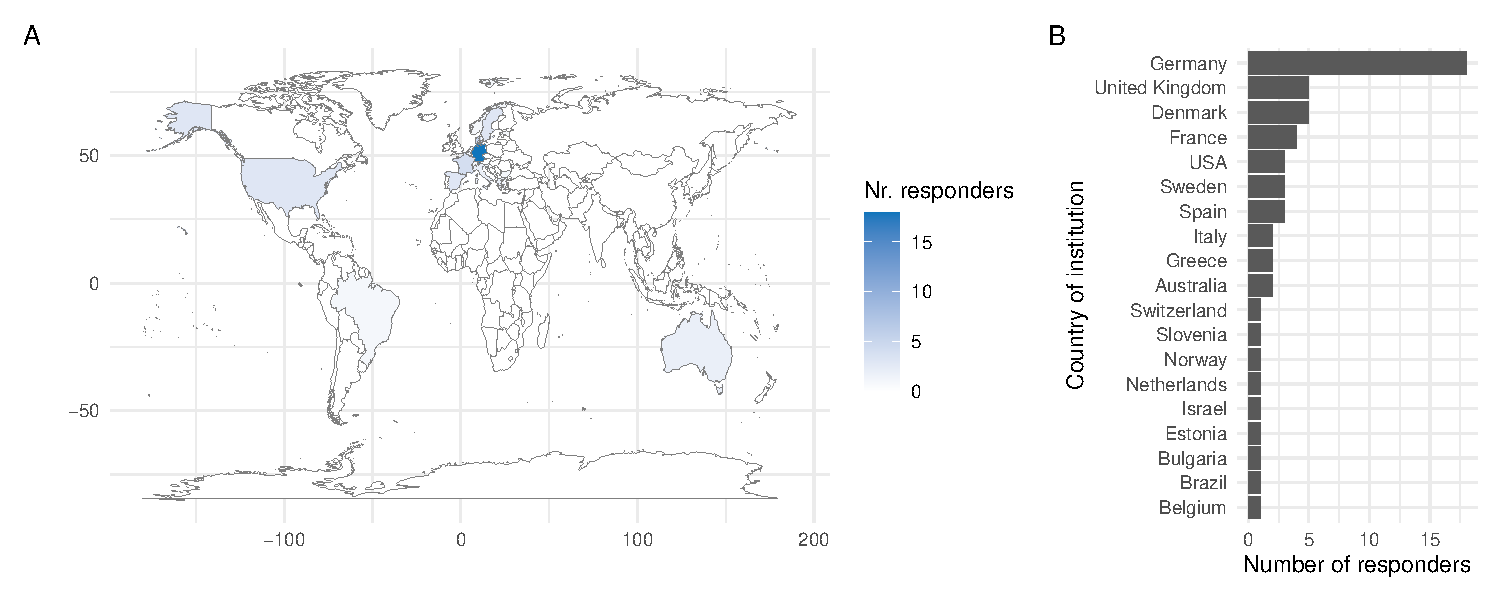
\includegraphics[keepaspectratio]{mixs-ux-survey_files/figure-pdf/unnamed-chunk-4-1.pdf}}

The vast majority of responders come out of European countries, and
other similar richer countries (USA, Australia, Israel). Again the
largest portion of responders come out of Germany, reflecting the
visibility of the survey to NFDI4Microbiota-associated researchers.

We asked what career state the responder was in, and if they were
associated with any relevant MIxS consortia.

\pandocbounded{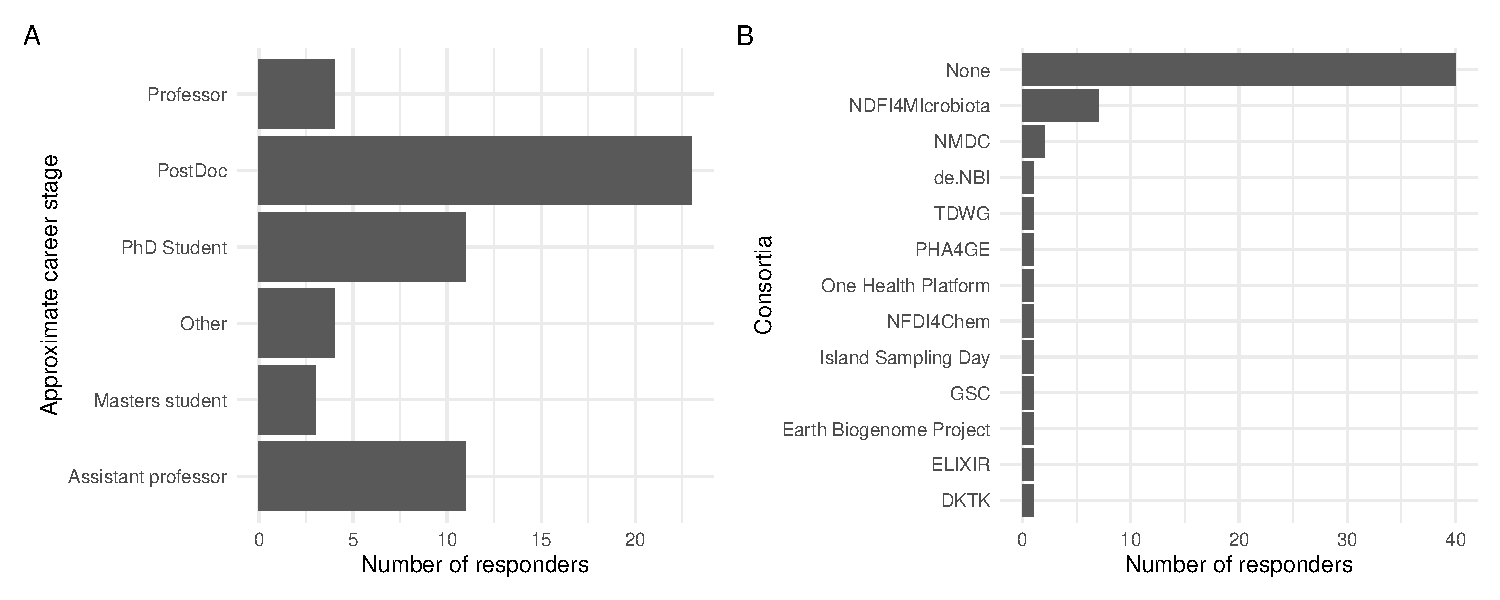
\includegraphics[keepaspectratio]{mixs-ux-survey_files/figure-pdf/unnamed-chunk-5-1.pdf}}

Most responders were later in academic career stage, either as Post Docs
or assistant professor stages. Most responders were not associated with
a particular consortia, but NFDI4Microbiota and the National Microbiome
Data Collaborative (NMDC), who are both heavy users/investors in the
MIxS project were at the highest level.

The fields that the responders worked in were:

\pandocbounded{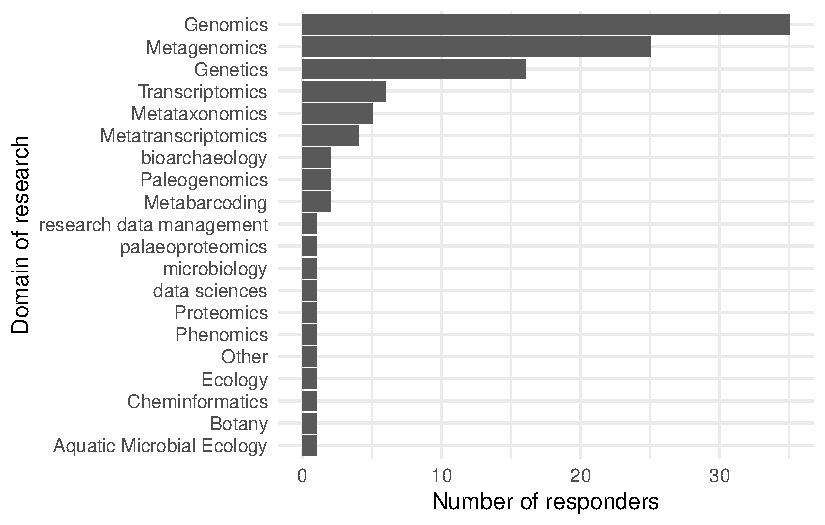
\includegraphics[keepaspectratio]{mixs-ux-survey_files/figure-pdf/unnamed-chunk-6-1.pdf}}

Most responders work in some form of (meta)genomics or handling
sequencing data, reflecting the primary advertising locations
(NFDI4Microbiota, Genomic Standards Consortium) - both of which have a
heavy focus on microbial genomics.

\subsubsection{Basic Questions}\label{basic-questions}

To get a better idea in which context the responders were providing
feedback from, we first asked whether the responders have in the past,
or were currently, handling forms of nucleic acid sequencing data.

\pandocbounded{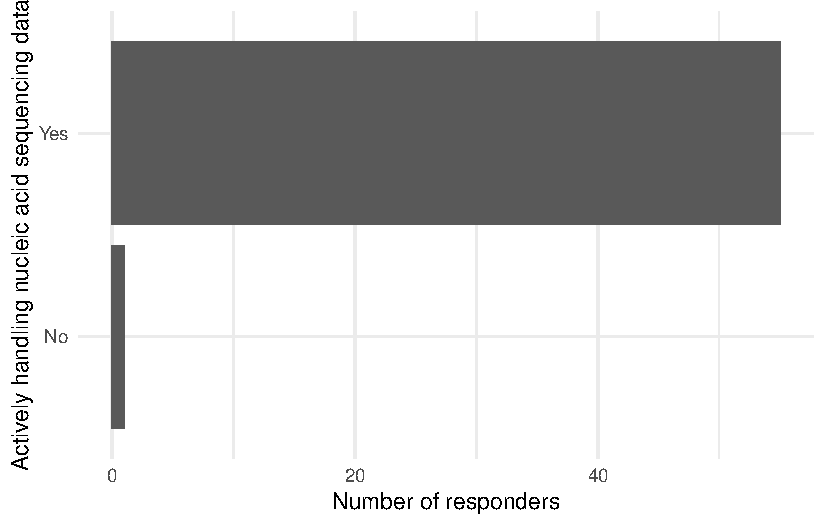
\includegraphics[keepaspectratio]{mixs-ux-survey_files/figure-pdf/unnamed-chunk-7-1.pdf}}

The \textbf{98.2\%} of 56 responders were/are handling sequencing data
now or in the past, as expected in terms of people who would be
interested in working on or contributing to improving metadata
annotation quality of sequencing data.

Of those who were handling data, we then asked if within the context of
their work, they had heard of the MIxS project and where they had heard
of it initially.

\pandocbounded{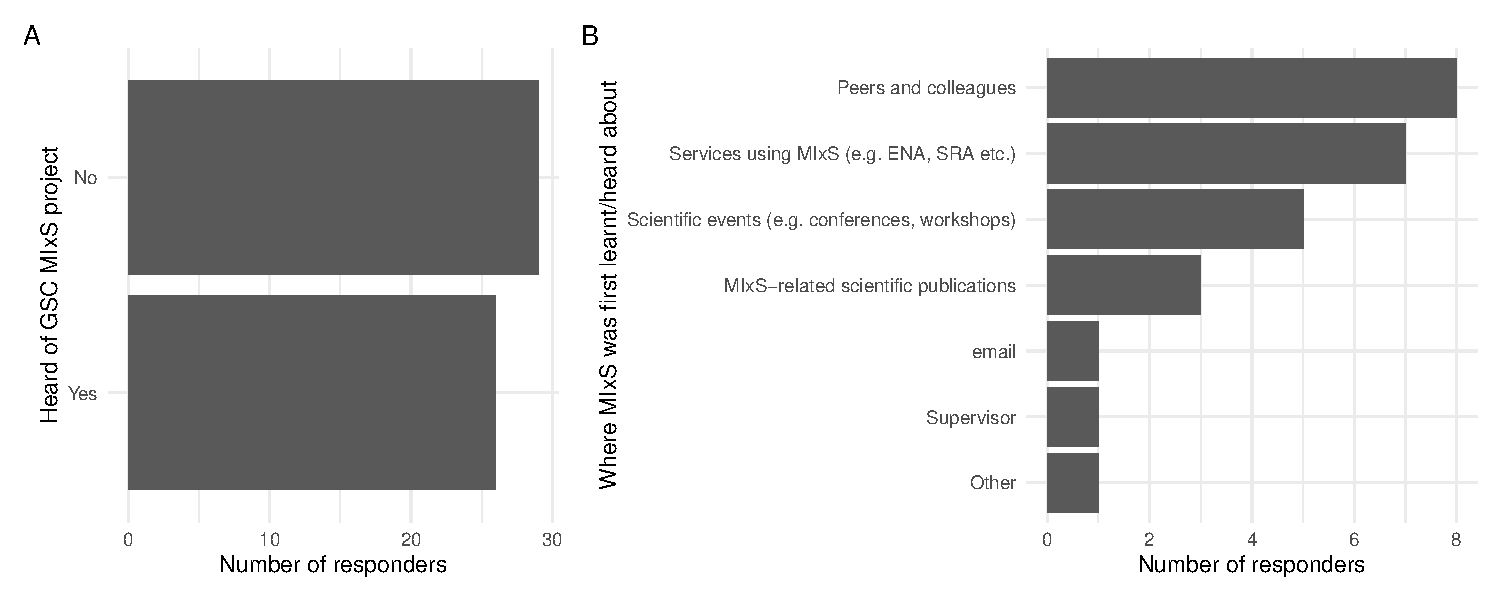
\includegraphics[keepaspectratio]{mixs-ux-survey_files/figure-pdf/unnamed-chunk-8-1.pdf}}

Only \textbf{47.3\%} of 55 had heard of the MIxS project.

This is a useful metric, as we can therefore see that despite many
researchers are handling sequencing data, less than half have heard of a
metadata standards project that has been around since 2008 (MIGS) or
2011 (MIxS), despite adoption by major sequencing data repositories such
as NCBI's SRA and EBI's ENA. An awareness campaign could be useful in
this regard, also to attract in new contributors and refresh the
project's working groups.

This is particularly as the project is mostly known via word of mouth or
through exposure during data upload.

More specifically, if discovered via a publication, event, or social
media, these venues were:

{\def\LTcaptype{none} % do not increment counter
\begin{longtable}[]{@{}
  >{\raggedright\arraybackslash}p{(\linewidth - 0\tabcolsep) * \real{1.0000}}@{}}
\toprule\noalign{}
\begin{minipage}[b]{\linewidth}\raggedright
Source of discovery
\end{minipage} \\
\midrule\noalign{}
\endhead
\bottomrule\noalign{}
\endlastfoot
An online presentation by James Fellows Yates in 2023, I think. \\
ENA and SRA \\
it was so long ago I dont recall! \\
https://doi.org/10.1038/nbt.1823 \\
AEGIS meeting Helsinborg \\
I think it was from the first publication, of Yilmaz et al.~At the time,
I had generated sequencing data (FLX) and I was about to submit them to
ENA. \\
\end{longtable}
}

With the DOI being the original Yilmaz et al.~(2011) paper in the
journal Nature Biotechnology.

Only two of the people who remembered how they found MIxS were from
events. However we asked responders if they had attended any GSC
conference or event at all.

\pandocbounded{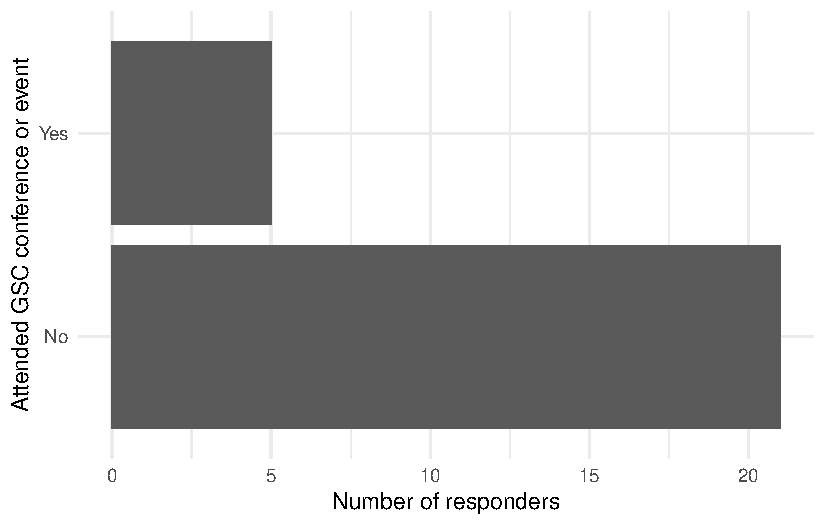
\includegraphics[keepaspectratio]{mixs-ux-survey_files/figure-pdf/unnamed-chunk-10-1.pdf}}

Of 26 responders \textbf{19.2\% }have attended a GSC conference or
event. This is not to be unexpected as likely GSC conferences or events
are more likely to be heavier users or developers, as the events have
been generally aimed at researchers with a strong interest in metadata
standards.

\subsubsection{Usage of MIxS}\label{usage-of-mixs}

We next asked whether the responders who handled nucleic acid sequencing
data and had heard of MIxS about their usage of MIxS itself (not just
awareness of the project), whether using a checklist or developing one.

\pandocbounded{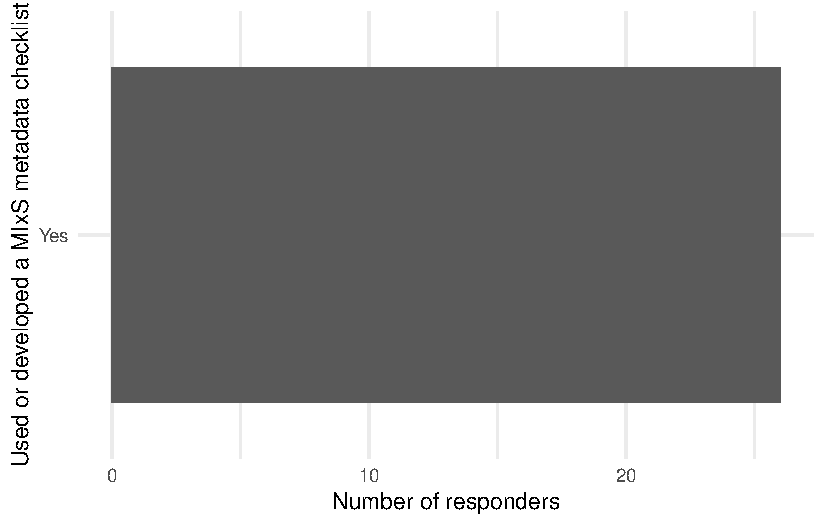
\includegraphics[keepaspectratio]{mixs-ux-survey_files/figure-pdf/unnamed-chunk-11-1.pdf}}

Of the remaining responders (26), \textbf{100\%} had interacted with
MIxS in some form.

The breakdown of the interactions are as follows:

\pandocbounded{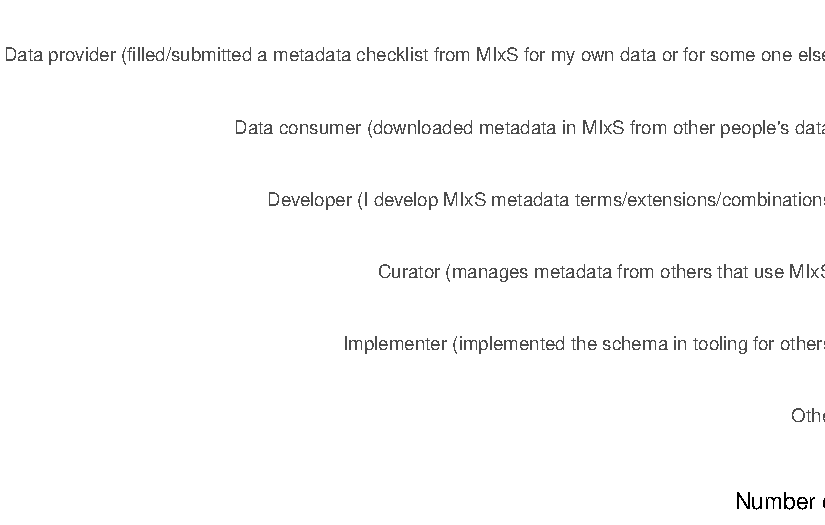
\includegraphics[keepaspectratio]{mixs-ux-survey_files/figure-pdf/unnamed-chunk-12-1.pdf}}

Most responders have been submitting or processing existing metadata,
with only a smaller fraction actually developing or implementing the
standard's schemas themselves.

We asked those who had been submitting or processing the metadata, where
the primary location of such interactions were.

\pandocbounded{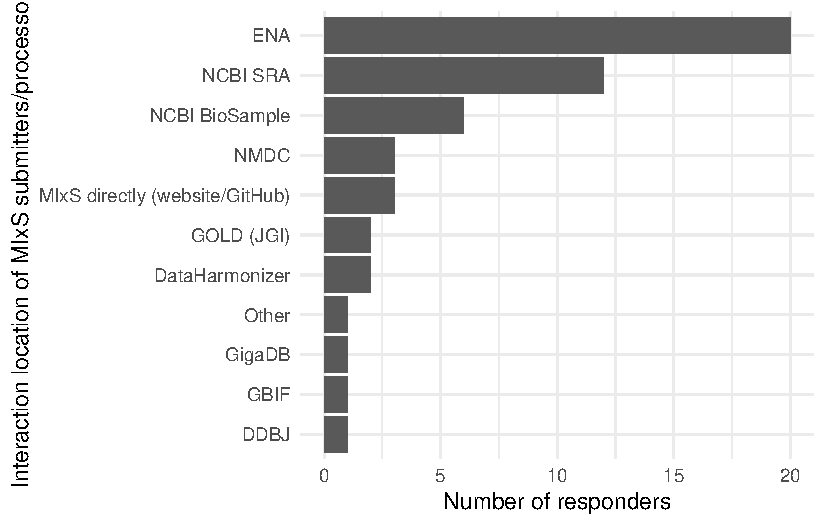
\includegraphics[keepaspectratio]{mixs-ux-survey_files/figure-pdf/unnamed-chunk-13-1.pdf}}

As expected, the vast bulk of the responders were interacting with
databases associated with the INSDC consortium of sequencing data
repositories (ENA, and NCBI).

To get an idea in which ways metadata submitters/processing are actually
handling the metadata themselves (filling in, validation, etc.), we
asked if they have used a validation tool, and if so which methods and
tools they are using.

\pandocbounded{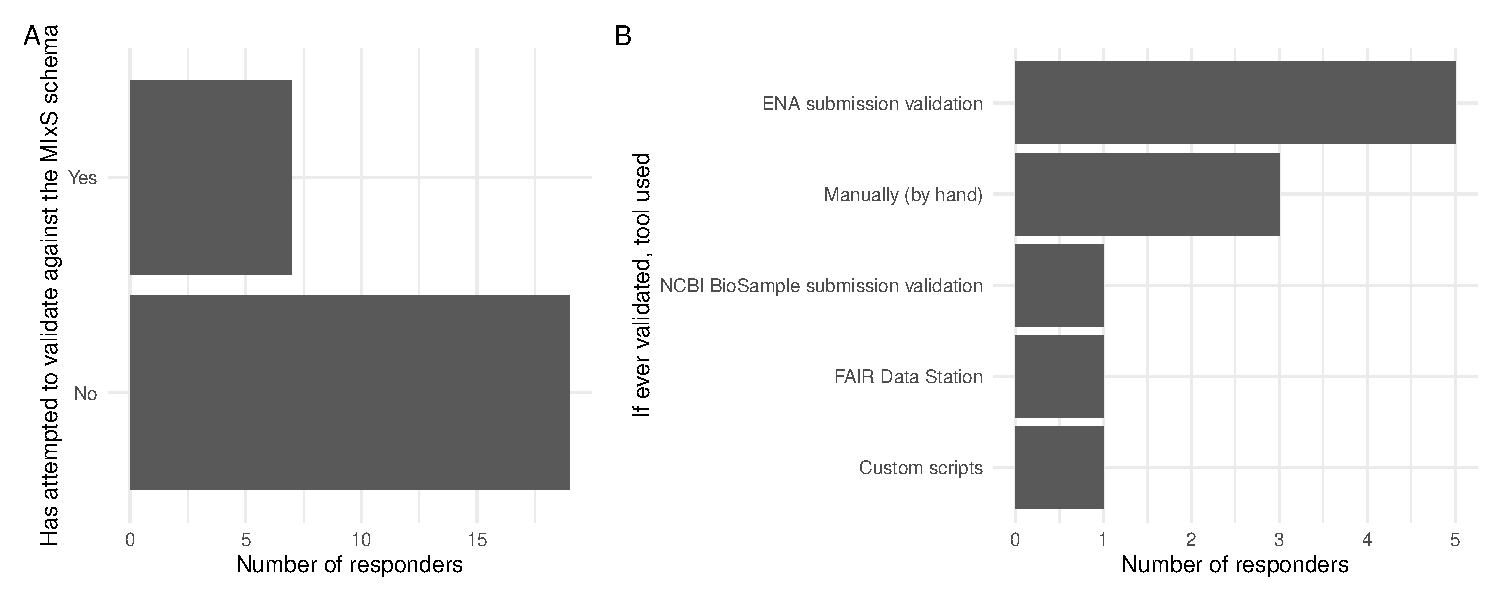
\includegraphics[keepaspectratio]{mixs-ux-survey_files/figure-pdf/unnamed-chunk-14-1.pdf}}

Very few of the responders (\textbf{7}) have actively have tried to
validate metadata, and of those most of these were using the ENA
submission form (reflecting the European centric make up of responders)
or manually (e.g.~using custom scripts).

The MIxS developers were also interested to know whether researchers
using the validation tools felt they were validating correctly - i.e.,
the validators checked the submitted metadata in the way they understood
MIxS defined each term.

\pandocbounded{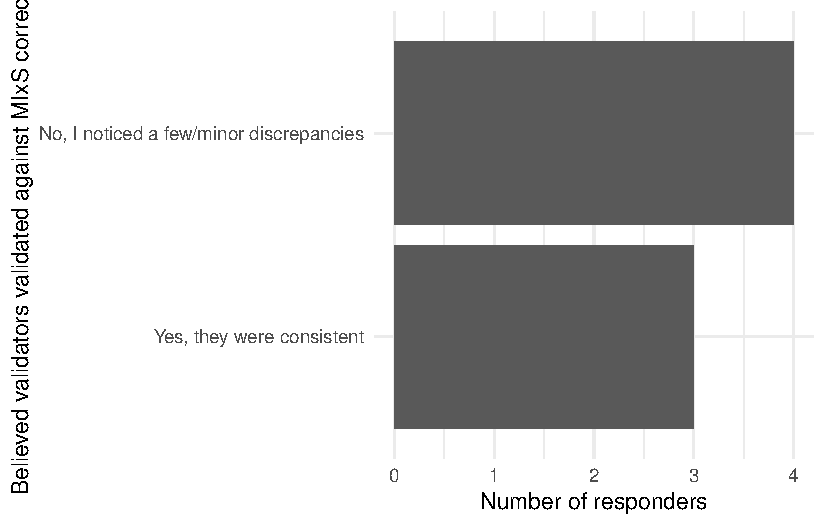
\includegraphics[keepaspectratio]{mixs-ux-survey_files/figure-pdf/unnamed-chunk-15-1.pdf}}

Even though there were few responders, approximately half felt the tools
were not always validating correctly.

{\def\LTcaptype{none} % do not increment counter
\begin{longtable}[]{@{}lr@{}}
\toprule\noalign{}
fields & count \\
\midrule\noalign{}
\endhead
\bottomrule\noalign{}
\endlastfoot
Custom scripts & 1 \\
FAIR Data Station & 1 \\
NCBI BioSample submission validation & 1 \\
ENA submission validation & 2 \\
Manually (by hand) & 2 \\
\end{longtable}
}

Despite the small sample-size, the perceived discrepancies between the
the validation tools output and the MIxS schema itself, it appears these
occur across all validation tools.

\subsubsection{Knowledge of MIxS}\label{knowledge-of-mixs}

We next wanted to understand how much the responders knew of the MIxS
standard, including core concepts and about the main checklists
themselves.

We first wanted to know the locations, if any, that the responders would
read to get more information about MIxS.

\pandocbounded{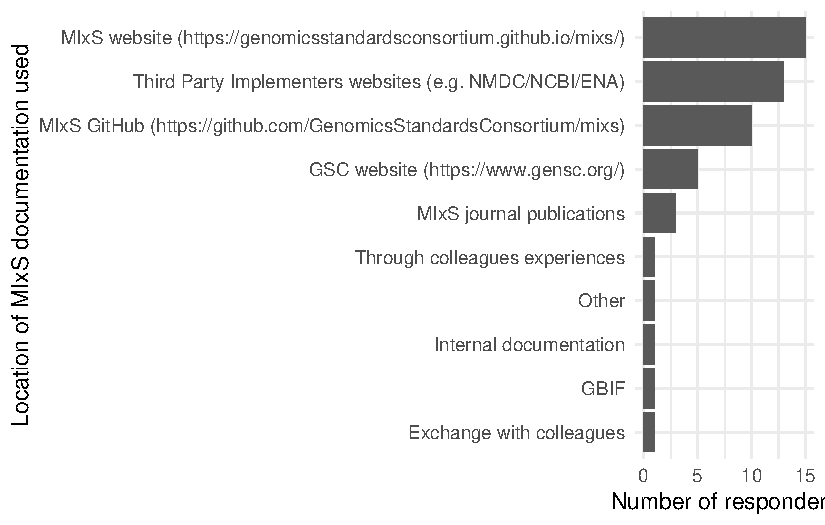
\includegraphics[keepaspectratio]{mixs-ux-survey_files/figure-pdf/unnamed-chunk-17-1.pdf}}

The majority of responders to this question (\textbf{26}) refer to
either the official/central MIxS website, the MIxS GitHub, or use data
repository websites to get information on the MIxS standard.

We then asked if responders were aware of the core MIxS concepts of
terms, checklists, and extensions.

\pandocbounded{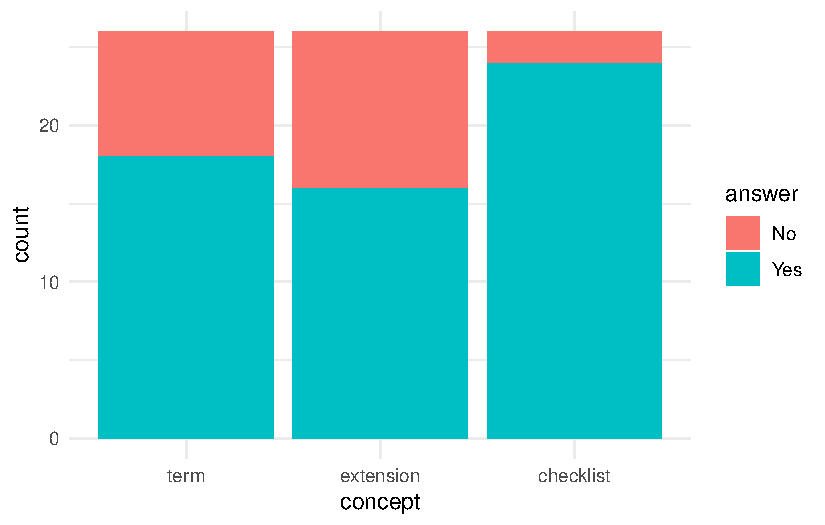
\includegraphics[keepaspectratio]{mixs-ux-survey_files/figure-pdf/unnamed-chunk-18-1.pdf}}

We see that the the concept of a MIxS checklist, is the most well known
(i.e, the full collection of terms for a specific sample type), however
the more granular components are less well known.

Similarly, we wanted to gauge approximately what were the more popular
`core' checklists and extensions, that generally represents the type of
sequencing data being annotated, and the type of samples, respectively.

\pandocbounded{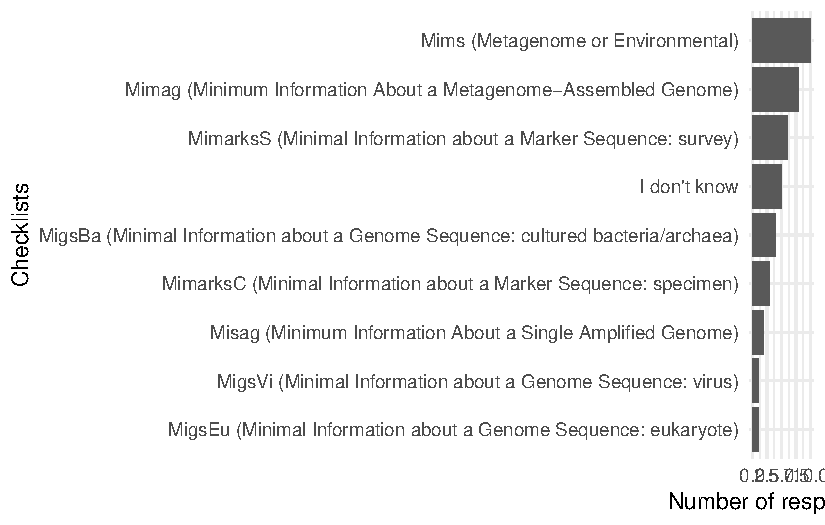
\includegraphics[keepaspectratio]{mixs-ux-survey_files/figure-pdf/unnamed-chunk-19-1.pdf}}

The most common checklists used were those associated with microbial
ecology, partly reflecting the fields in which MIxS was generated from,
as well as the networks that the author circulated the survey.

We asked the same question for that of extensions.

\pandocbounded{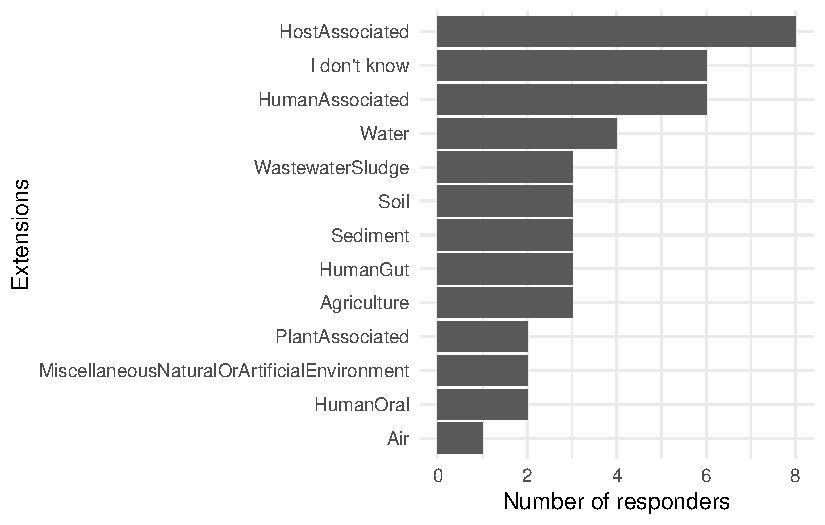
\includegraphics[keepaspectratio]{mixs-ux-survey_files/figure-pdf/unnamed-chunk-20-1.pdf}}

Most researchers responders have been working primarily on host and/or
human associated data.

\subsubsection{Contributing to MIxS}\label{contributing-to-mixs}

To better understand impressions and experiences about contributing with
MIxS, we asked a range of questions related to how researchers and
collaborate or work directly on the project.

First we wanted to know how many of the responders were considering now
or in the near future contributing or updating an existing term.
Additionally, we want to know whether these responders would know knew
what the procedure would be for a community contribution.

\pandocbounded{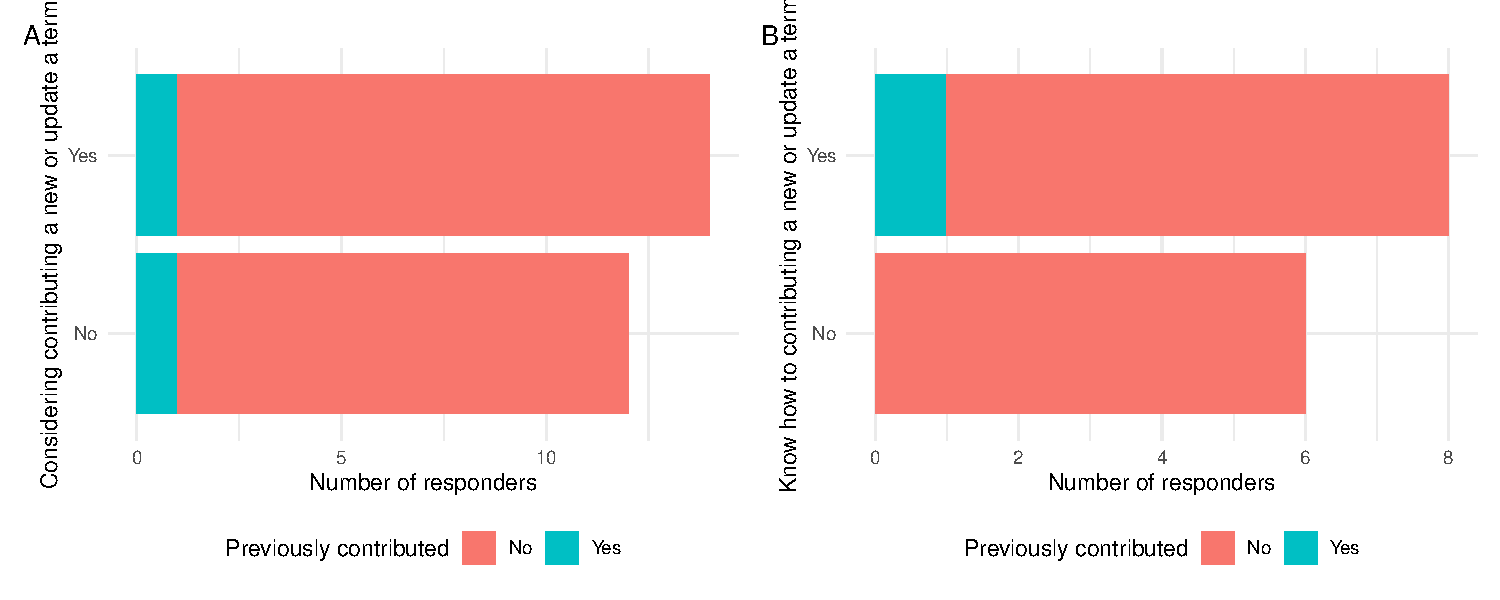
\includegraphics[keepaspectratio]{mixs-ux-survey_files/figure-pdf/unnamed-chunk-21-1.pdf}}

Of the responders that responded to the survey, and were familiar with
MIxS, more than half said they were considering now or in the new
future. Few of the responders had actually contributed or updated a MIxS
term previously. Of the 14 responders who were considering contributing
or updating an existing MIxS term, almost half did not know how they
would do so.

We then asked the same question however about contributing a new or
updating an existing extension.

\pandocbounded{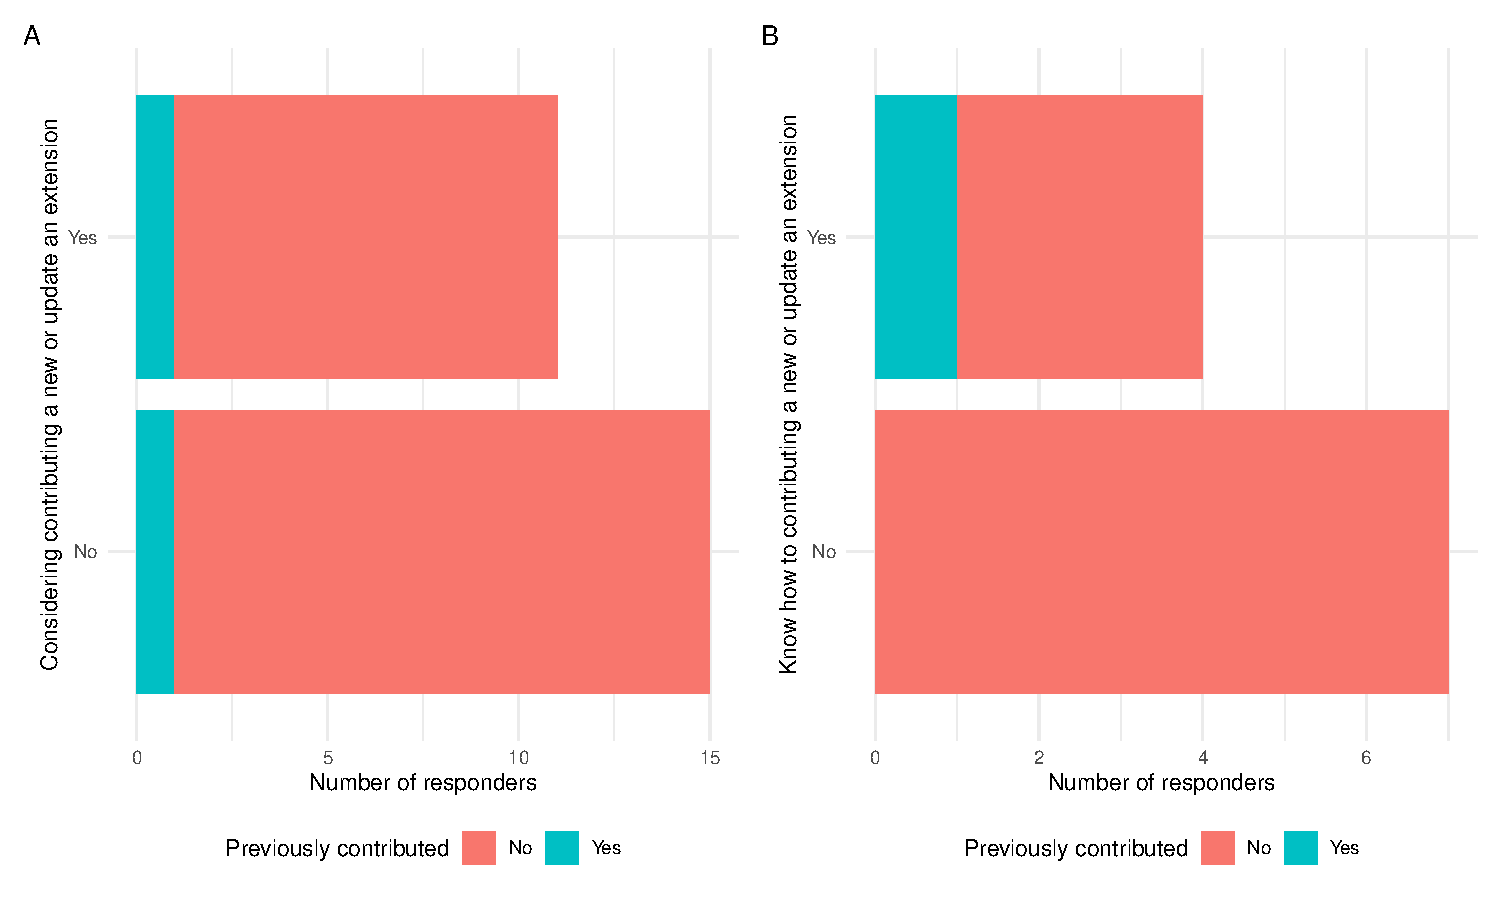
\includegraphics[keepaspectratio]{mixs-ux-survey_files/figure-pdf/unnamed-chunk-22-1.pdf}}

The distribution of Yes/No answers for both terms and also extensions
are mostly equivalent, with slightly less people planning on
contributing an extension knowing how the would do so.

Of the the 2 responders who had previously contributed, they had
contributed to:

\pandocbounded{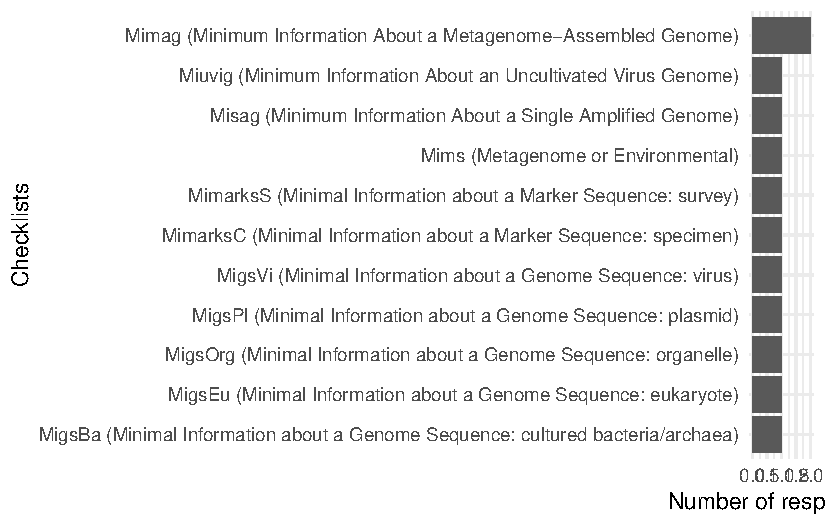
\includegraphics[keepaspectratio]{mixs-ux-survey_files/figure-pdf/unnamed-chunk-23-1.pdf}}

In this case one responder had contributed to all, suggesting the
responder as an original architect of the MIxS standard.

We asked for those who had previously you have contributed to MIxS, what
did they find was the hardest part?

As there were only two responders who had contributed previously to
MIxS, the numbers were low. One user found it difficult understanding
submission processes (who to contact, how to get approval, how to get
feedback, and how to submit the changes), whereas the other responder
did not understand the structure of the new LinkML MIxS based schema.

We also asked all responders familiar with MIxS that had considered to
contribute to MIxS, but didn't - what factors contributed to them not
doing so.

\pandocbounded{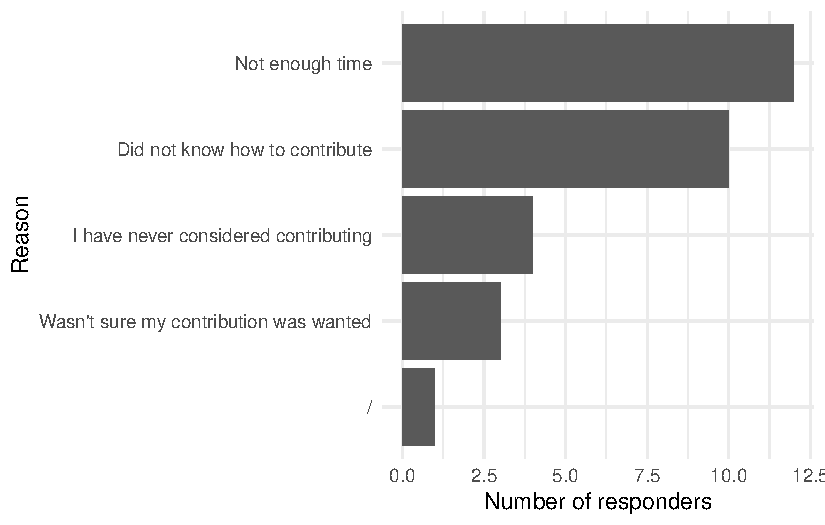
\includegraphics[keepaspectratio]{mixs-ux-survey_files/figure-pdf/unnamed-chunk-24-1.pdf}}

The two main reasons were time, but also similar to the feedback from
the existing contributors - not knowing how to contribute remains a big
issue.

\pandocbounded{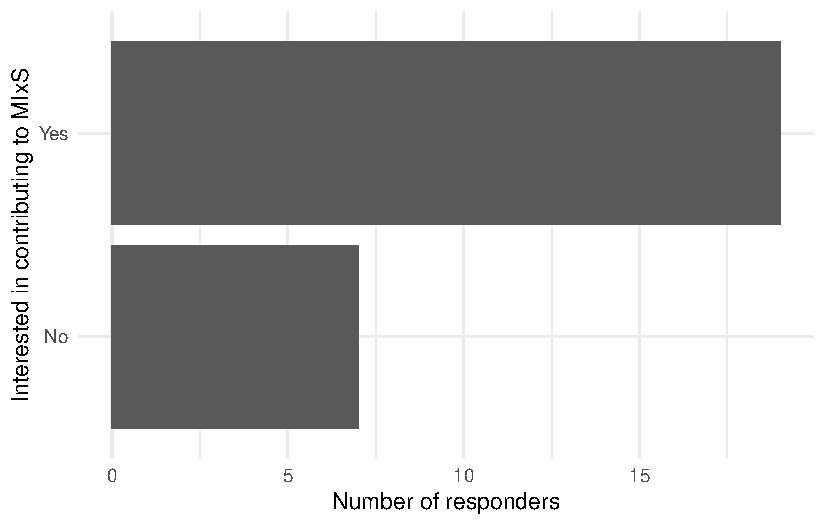
\includegraphics[keepaspectratio]{mixs-ux-survey_files/figure-pdf/unnamed-chunk-25-1.pdf}}

However, despite the high number of responders not previously
contributing, and a mixture of confidence in knowing how to contribute,
most responders familiar with MIxS are interested in getting involved in
developing the standard.

\subsubsection{Technical Questions}\label{technical-questions}

Due to the recent change of a custom schema system to the LinkML
framework (\href{https://dx.doi.org/10.1093/gigascience/giaf152}{Moxon
et al.~2026}), we were interested in getting a better idea of the
technical knowledge of the responders.

\pandocbounded{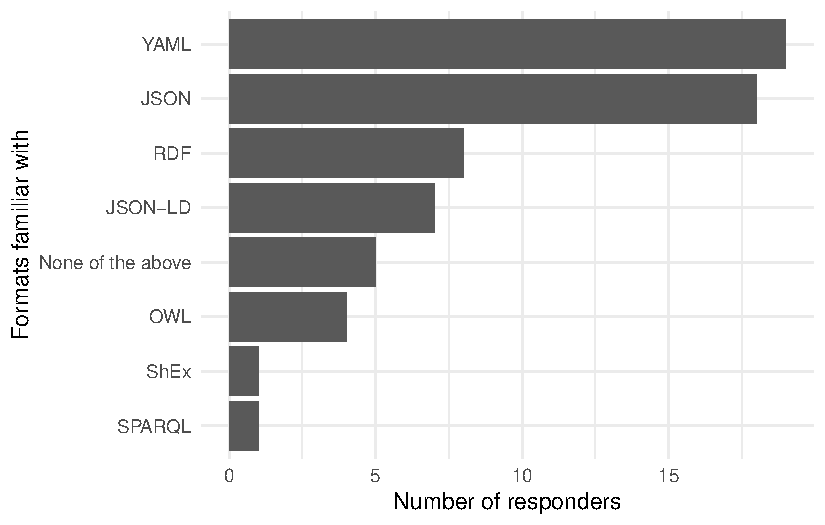
\includegraphics[keepaspectratio]{mixs-ux-survey_files/figure-pdf/unnamed-chunk-26-1.pdf}}

Common `generic' computational formats such as YAML or JSON that are
used across most software development and/or bioinformatics were most
well-known, whereas dedicated linked-data or schema formats were less
well known, likely as many genomics researchers handling metadata not
having had training specifically in metadata management.

We also asked specifically if responders knew that MIxS was now
implemented within LinkML, and thus can be converted to multiple
formats, and whether they had used such functionality and if so had it
helped their productivity with using MIxS

\pandocbounded{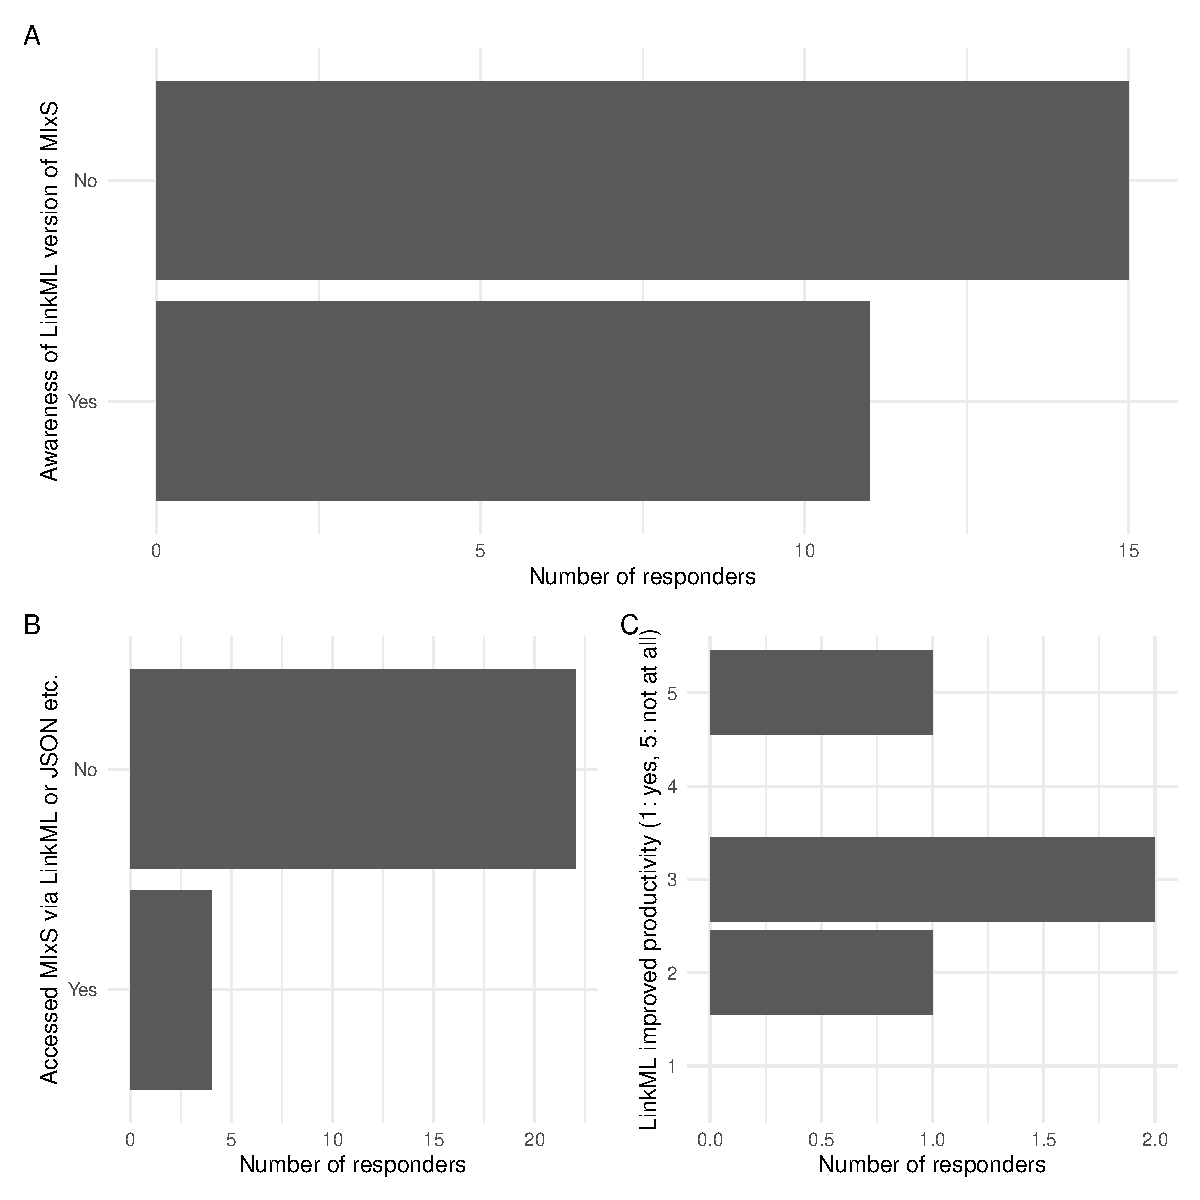
\includegraphics[keepaspectratio]{mixs-ux-survey_files/figure-pdf/unnamed-chunk-27-1.pdf}}

Just under half of responders knew about the LinkML version of MIxS, but
very few used this new functionality currently. However it has somewhat
helped the few users who had used it.

\subsubsection{Wider context}\label{wider-context}

Closing the survey, we asked if used other standards, and if so which
one.

To get wider feedback on the state of genomic metadata standards, we
also asked what the responders would like to see improved in other
standards.

\pandocbounded{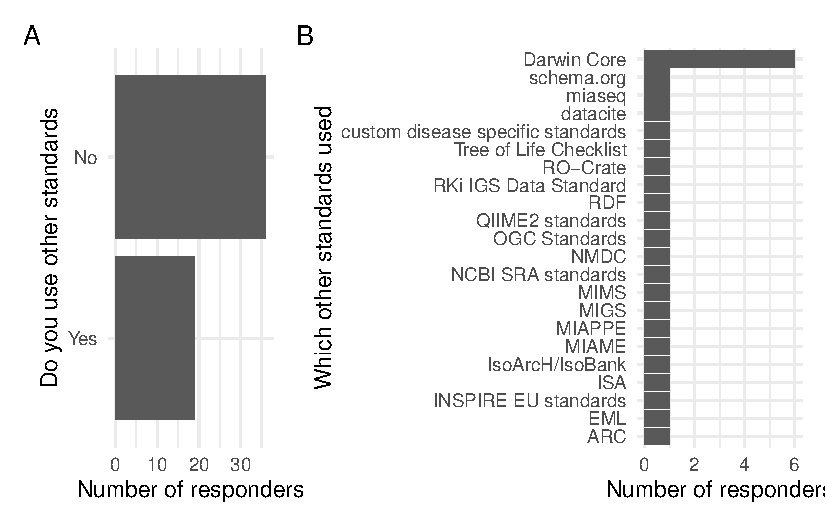
\includegraphics[keepaspectratio]{mixs-ux-survey_files/figure-pdf/unnamed-chunk-28-1.pdf}}

Most of the whole set of responders did not use other standards, and of
those that did, there was a wide range of metadata standards used - with
Darwin Core being the particular stand out.

Improvements desired in these other standards were varied, but a common
request was better interlinking between different standards.

{\def\LTcaptype{none} % do not increment counter
\begin{longtable}[]{@{}
  >{\raggedright\arraybackslash}p{(\linewidth - 0\tabcolsep) * \real{1.0000}}@{}}
\toprule\noalign{}
\begin{minipage}[b]{\linewidth}\raggedright
Any further comments
\end{minipage} \\
\midrule\noalign{}
\endhead
\bottomrule\noalign{}
\endlastfoot
No \\
Not now. \\
How to handle metadata following FAIR principles \\
It would be useful to link to other biomolecular data from the same
samples/individuals e.g.~radiocarbon, stable isotopes, palaeoproteomics
etc. for easier cross-referencing. \\
We we format our metadata in accordance with public repositories (ENA,
BOLD, NCBI) \\
Metadata could also be expanded to include (genome) assemblies and
(genome) annotations also. \\
I just wish mixs existed sooner! \\
\end{longtable}
}

\subsection{Discussion}\label{discussion}

In total we had 56 responders, mostly from `High-Income economy'
countries and with a strong European focus. As expected due to the
context of the standard, most responders worked within genomics,
metagenomics, and/or metatranscriptomics. \textbf{Interestingly, most
responders are working at a Post-doctoral level (or equivalent) or
higher career stage.} The reason for this is unclear, but could be
something that should be investigated further, could this be due to:

\begin{itemize}
\tightlist
\item
  A lack of training in metadata annotation?
\item
  A generational or visibility factor (e.g.~MIxS is now 20 years old)
\item
  Experience level (e.g.~many Ph.D.~students may not encounter
  annotating their data until upload at the end of their projects)
\item
  Expected responsibilities (e.g.~if metadata annotation/data upload is
  left to employees with more engineering roles)
\end{itemize}

Across all responders, only 50\% had heard of MIxS, and those who had
had mostly had learnt about the standards through word-of-mouth through
Peers or exposure from services implementing the standard. All
responders who had heard of MIxS had used it - mostly in the role of a
data uploader or downloader at INSDC repositories (EBI-ENA, NCBI-SRA
etc.). \textbf{This indicates that targeting `consumers' as potential
`starting points' maybe an ideal starting point in prioritising which
project documentation to developer, and could raise more interest in
contributing to the project.}

Most responders who were aware of MIxS indicated they primarily got
their information about MIxS from the MIxS GitHub repository
(\url{https://github.com/GenomicsStandardsConsortium/mixs}) and
associated project website
(\url{https://genomicsstandardsconsortium.github.io/mixs/}), or
third-party implementers such as ENA or SRA, rather than the GSC website
(\href{https://genomicsstandardsconsortium.github.io/mixs/}{https://www.gensc.org/})
or academic publications. \textbf{This therefore suggests that the most
suitable place for MIxS documentation would be on the MIxS GitHub
repository.}

In terms of familiarity with the project, almost all responders familiar
with MIxS understood what a MIxS \emph{checklist} was, however the
concepts of an \emph{extension} or \emph{term} were less well known.
\textbf{This suggests that information about basic MIxS concepts need to
be better described or more clearly placed to ensure understanding of
how the standard works at a fundamental level.}

The MIMS, MIMAG, and MIMARKS checklists from human or host-associated
samples were the most commonly used by responders. This likely reflects
the original history and background of the project, that primarily came
out of microbiology-related communities. \textbf{The popularity of MIMS,
MIMAG, and MIMARK checklists could be used to guide what types of
examples or training material could be developed in an improved MIxS
documentation framework, but also sources of potential test users of
such material.}

While the vast majority of responders have not previously contributed to
MIxS, more than a third were interested in doing so (either via a term
or extension). \textbf{The main factors for not previously contributing
was simply time or not knowing how to contribute (with a smaller number
not knowing whether they were welcome to do so).} For the small number
of responders (2) who had previously contributed, their largest
obstacles had been an unclear submission process and being unfamiliar
with the new LinkML schema framework MIxS recently transition to. This
was reflected with less than half of the responders knowing about this
transition, and thus are potentially unaware of the benefits.
\textbf{Despite these factors, the vast majority of responders were
still interested in contributing to MIxS in some form - highlighting the
relevancy of the project and it's aims to responders.}

A common forward-looking feedback given by multiple responders was an
interest in seeing more interoperability and alignment between different
standards, with the Darwin Core metadata standard being the most popular
non-MIxS standard being utilised by responders.

\subsection{Acknowledgements}\label{acknowledgements}

This report was supported by the NFDI4Microbiota Flexfund `MIxS-UX',
funded by the Deutsche Forschungsgemeinschaft (DFG, German Research
Foundation) -- 460129525.




\end{document}
